\documentclass[xcolor=table]{beamer}
\beamertemplatenavigationsymbolsempty
\setbeamertemplate{blocks}[rounded=true, shadow=true]
\setbeamertemplate{footline}[page number]
\usecolortheme{beaver}

\usepackage{fontspec}
% enable the traditional TeX ligatures:
\defaultfontfeatures{Ligatures=TeX}
\setmainfont{Times New Roman}
\setsansfont{Arial}
\setmonofont[Script=Cyrillic]{DejaVu Sans Mono}

\newfontfamily\cyrillicfont{Times New Roman}
\newfontfamily\cyrillicfontsf{Times New Roman}

\usepackage{unicode-math}
\setmathfont{TeX Gyre Termes Math} 

\usepackage{polyglossia}
\setmainlanguage{russian}
\setotherlanguage{english}

\usepackage[backend=biber, style=authoryear, url=false, isbn=false]{biblatex}
\addbibresource{references.bib}

\usepackage{amssymb,amsfonts,amsmath}
\usepackage{algorithmic}
\usepackage{subfig}
\usepackage[all]{xy}
\usepackage{array}
\usepackage{tikz}
\usepackage{multicol}
\usepackage{hyperref}
\usepackage{hhline}
\graphicspath{{fig/}{../fig/}}

\DeclareMathOperator*{\argmax}{arg\,max}
\DeclareMathOperator*{\argmin}{arg\,min}


% A handy helper to put four graphics in a 2×2 grid (no extra packages needed).
% Usage: \quadgraphics{file1}{file2}{file3}{file4}
\newcommand{\quadgraphics}[4]{%
  \begin{columns}[T,onlytextwidth]
    \column{0.48\textwidth}
      \includegraphics[width=\linewidth]{#1}\\[0.5em]
      \includegraphics[width=\linewidth]{#3}
    \column{0.48\textwidth}
      \includegraphics[width=\linewidth]{#2}\\[0.5em]
      \includegraphics[width=\linewidth]{#4}
  \end{columns}}

%----------------------------------------------------------------------------------------------------------
\title{Эквифинальность в задачах гидрологического прогнозирования}
\author[Э. Хузин]{Эльдар Хузин}
\institute{Московский физико-технический институт}
\date{\footnotesize
  \emph{Консультант:} Д.~Абрамов\\
  2025
}

\begin{document}

\begin{frame}[plain]
    \maketitle
\end{frame}
%-----------------------------------------------------------------------------------------------------
\begin{frame}{Цель исследования}
    \begin{block}{Цель}
        Исследовать эквифинальность моделей RF, XGBoost, LSTM, а также их способность выявлять гидрологические закономерности в данных о стоке рек.
    \end{block}

    \begin{block}{Задачи}
        \begin{enumerate}
            \item Сравнить модели по метрикам NSE, RMSE, MAE, MAPE.
            \item Построить ``карту эквифинальности'' --- области, где ошибки моделей
                  статистически неразличимы.
            \item Оценить вклад признаков через SHAP-значения.
            \item Проанализировать компромисс ``точность\textbackslash вычислительная
                  сложность\textbackslash интерпретируемость''.
        \end{enumerate}
    \end{block}

    \begin{block}{Решение}
        Провести на обширном датасете временных рядов и статических признаков SHAP--анализ моделей.
    \end{block}
\end{frame}

%----------------------------------------------------------------------------------------------------------
\begin{frame}{Публикации по теме}
    \nocite{
        bevenFutureDistributedModels1992a,
        schmidtChallengesApplyingMachine2020
        underwoodMachineLearningRevealsEquifinality2023,
        janssenTacklingWaterTable2024,
        SpatialtemporalBehaviorPrecipitation2022,
    }
    \printbibliography[heading=None]
\end{frame}

%----------------------------------------------------------------------------------------------------------
\begin{frame}{Вычислительный эксперимент}
    \begin{enumerate}
        \item Предобработка данных
              \begin{enumerate}
                  \item Корреляционный анализ и отбор статических признаков
                  \item Заполнение пропусков
                  \item Добавление лагов и статических атрибутов
              \end{enumerate}
        \item Обучение
              \begin{enumerate}
                  \item Выделение выборок (12/3)
                  \item Подбор гиперпараметров
                  \item Обучение
              \end{enumerate}
        \item SHAP-анализ и другие метрики    \[
                  \phi_i=\!\!\!\sum_{S\subseteq N\setminus\{i\}}
                  \frac{|S|!\,(|N|-|S|-1)!}{|N|!}\;
                  \bigl[f(S\cup\{i\})-f(S)\bigr]
              \]
    \end{enumerate}
\end{frame}


%----------------------------------------------------------------------------------------------------------
\begin{frame}{Данные}
    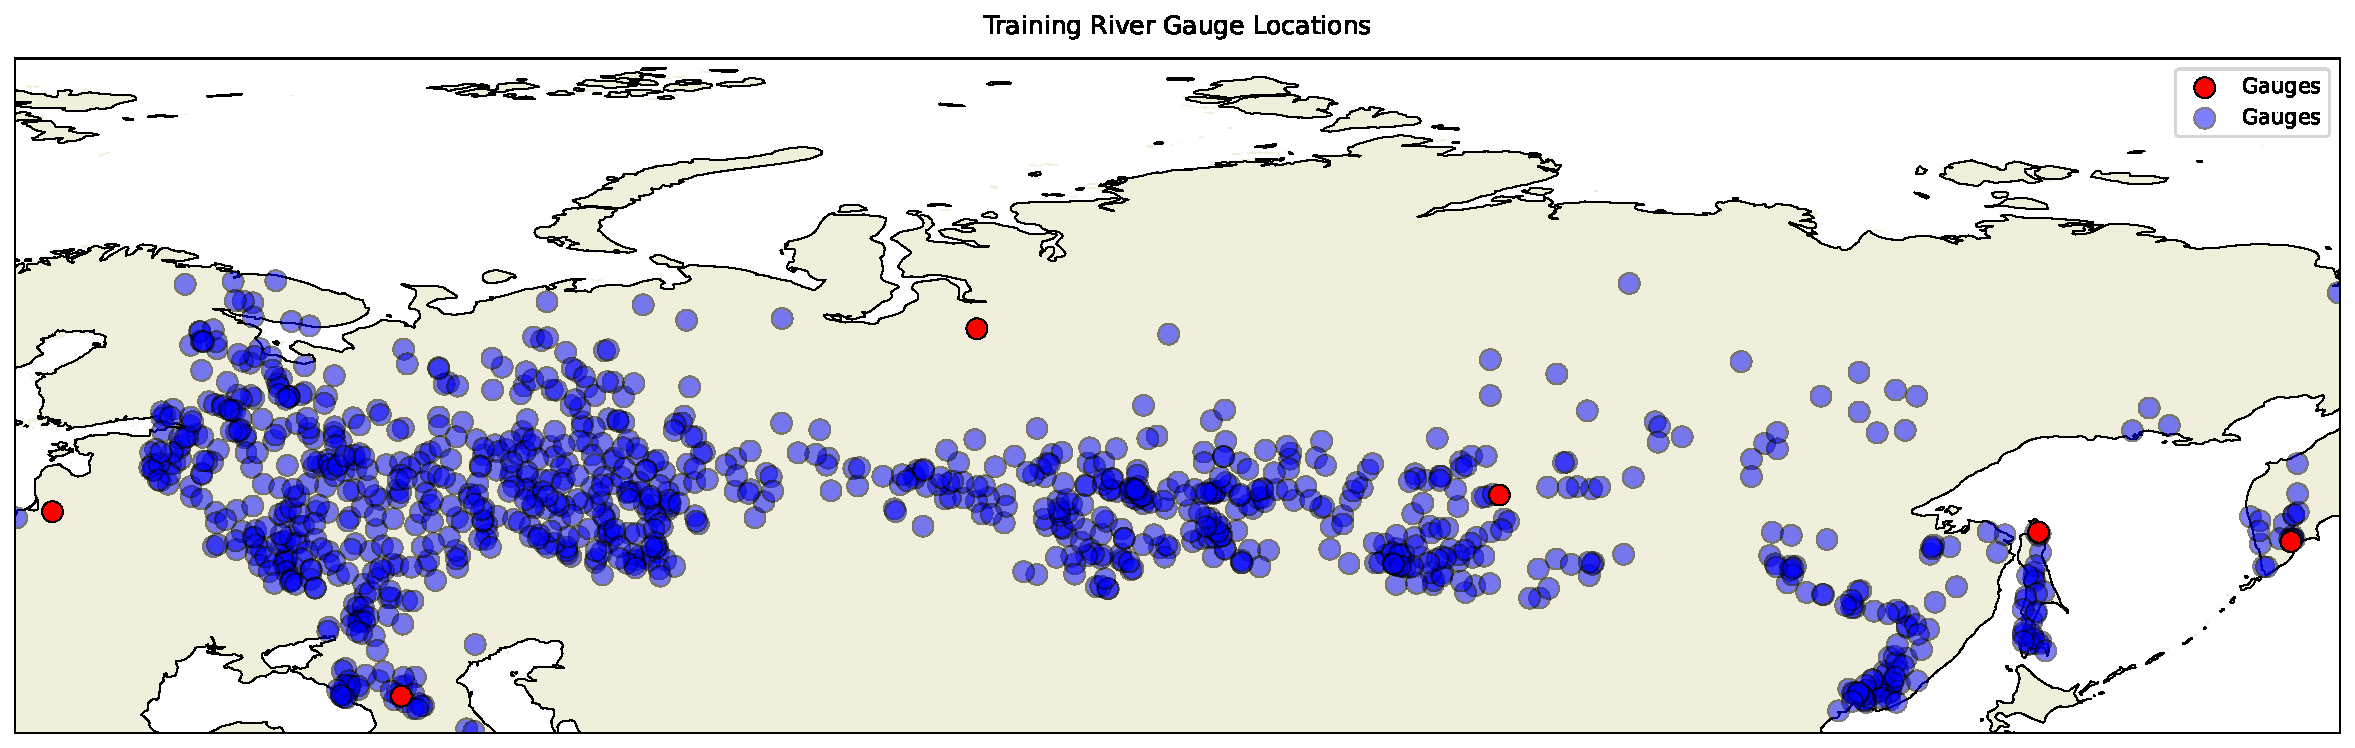
\includegraphics[width=1\textwidth]{bin/train_gauges_cartopy_10m_large.pdf}
\end{frame}

%----------------------------------------------------------------------------------------------------------
\begin{frame}{Данные}
    Ежедневные данные за период с 2008 по 2022 год на 1072 бассейнов.

    \medskip
    \textbf{prcp} – количество осадков (мм/сут)\\
    \textbf{lvl\_sm} – уровень воды в реке (м)\\
    \textbf{t\_min} – минимальная температура (°C)\\
    \textbf{t\_max} – максимальная температура (°C)\\
    \textbf{t\_mean} – средняя температура (от почасовой) (°C)\\
    \textbf{q\_mm\_day} – расход воды (мм/сут)\\
\end{frame}

\begin{frame}{Данные}
    
\includegraphics[width=1\textwidth]{bin/target_time_series.pdf}
\end{frame}

%----------------------------------------------------------------------------------------------------------
\begin{frame}{Описание атрибутов}
    \begin{table}[ht]
        \centering
        \begin{tabular}{lll}
            \toprule
            \textbf{ID}  & \textbf{Атрибут}                     &                       \\
            \midrule
            \textbf{L07} & Лесные территории (\%)               & \texttt{for\_pc\_sse} \\
            \textbf{L08} & Сельскохозяйственные угодья (\%)     & \texttt{crp\_pc\_sse} \\
            \textbf{L09} & Пастбища (\%)                        & \texttt{pst\_pc\_sse} \\
            \textbf{L10} & Орошаемые земли (\%)                 & \texttt{ire\_pc\_sse} \\
            \textbf{A03} & Урбанизированные территории (\%)     & \texttt{urb\_pc\_sse} \\
            \textbf{S07} & Карстовые ландшафты (\%)             & \texttt{kar\_pc\_sse} \\
            \textbf{P01} & Средняя высота над уровнем моря (м)  & \texttt{ele\_mt\_sav} \\
            \textbf{P02} & Средний уклон местности (°)          & \texttt{slp\_dg\_sav} \\
            \textbf{C06} & Аридность                            & \texttt{ari\_ix\_sav} \\
            \textbf{H10} & Глубина залегания грунтовых вод (см) & \texttt{gwt\_cm\_sav} \\
            \textbf{S05} & Среднегодовая влажность почвы (\%)   & \texttt{swc\_pc\_syr} \\
            \textbf{S01} & Глина в почве (\%)                   & \texttt{cly\_pc\_sav} \\
            \textbf{A06} & Индекс антропогенного воздействия    & \texttt{hft\_ix\_s09} \\
            \textbf{P04} & Географическая широта (°)            & \texttt{lat}          \\
            \textbf{P05} & Географическая долгота (°)           & \texttt{lon}          \\
            \bottomrule
        \end{tabular}
    \end{table}
\end{frame}


%----------------------------------------------------------------------------------------------------------
\begin{frame}{Данные}
    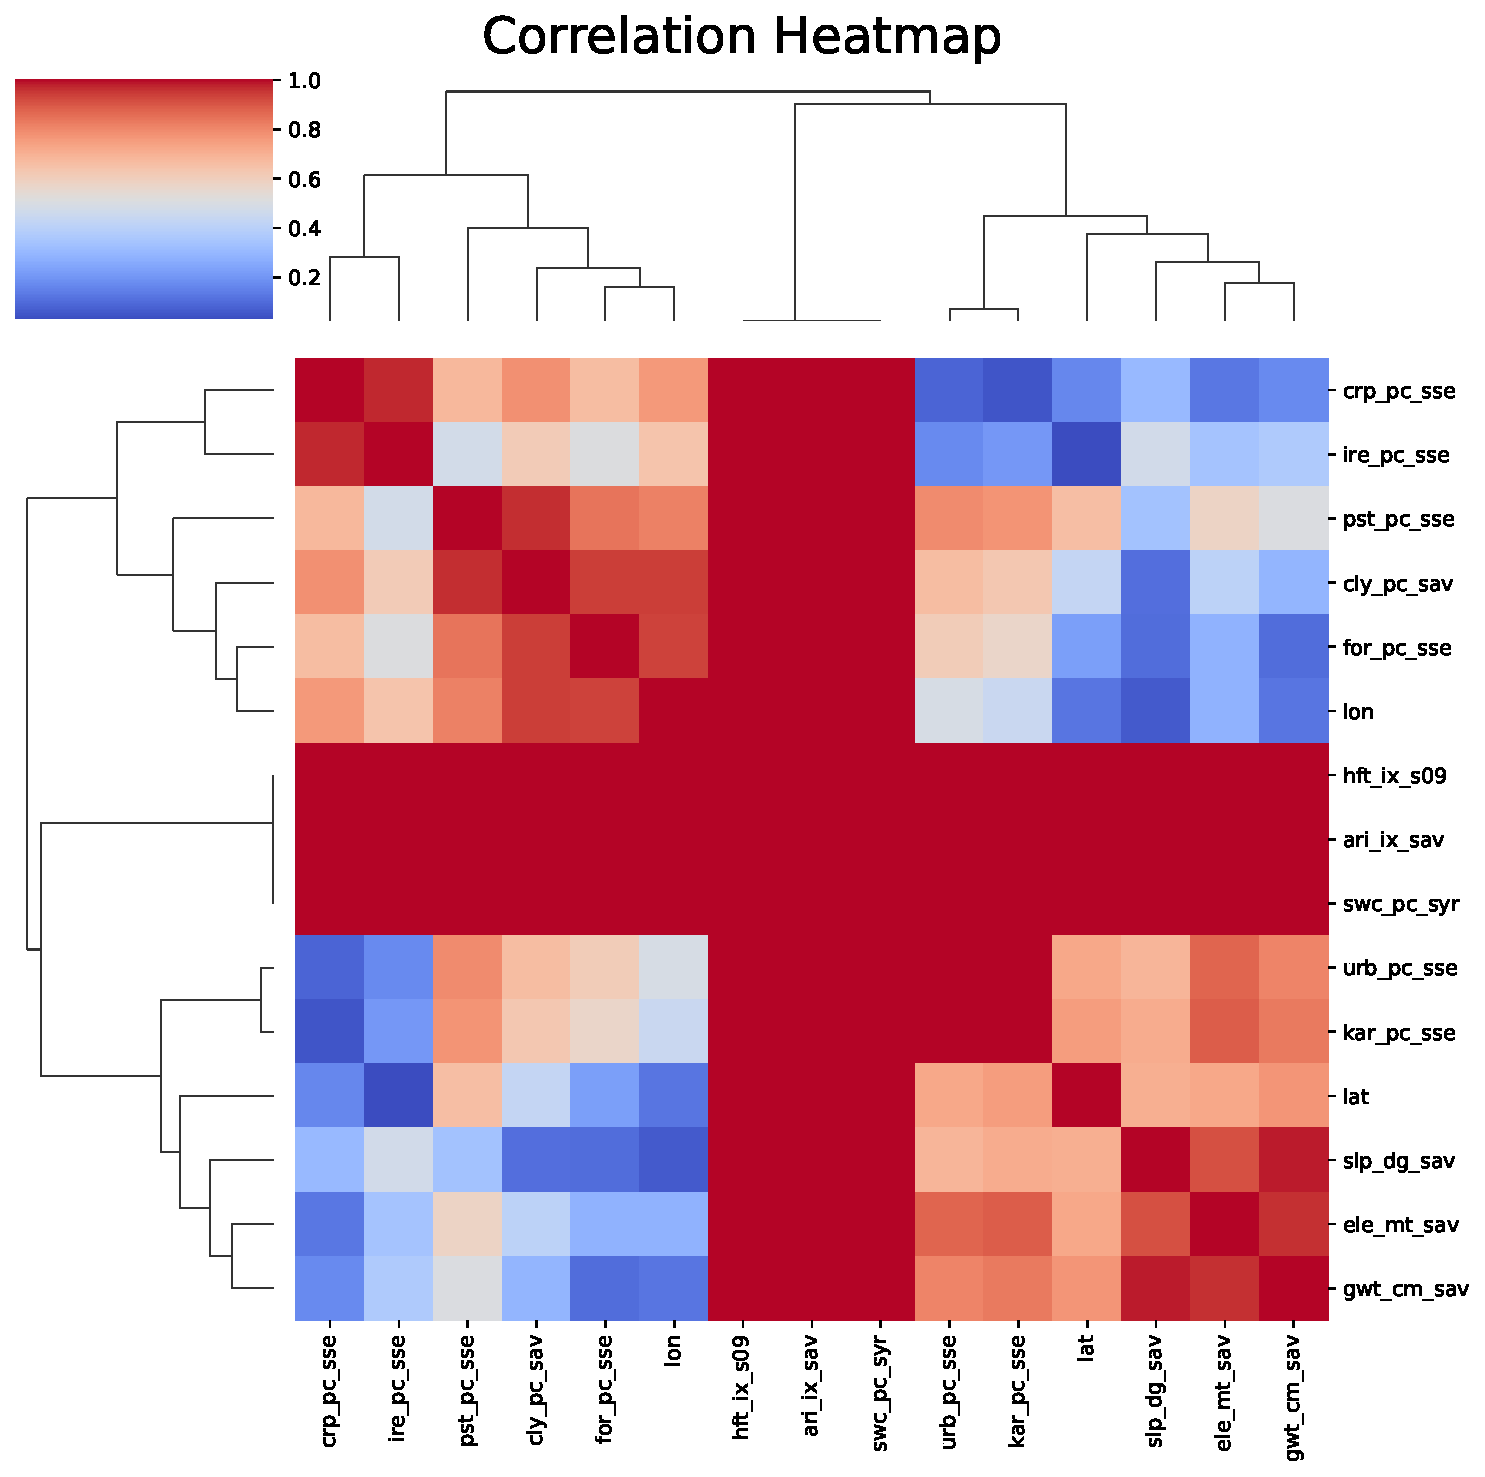
\includegraphics[height=0.7\textwidth]{bin/static_selected_features_heatmap.pdf}
\end{frame}

%----------------------------------------------------------------------------------------------------------
\begin{frame}{Формальная постановка задачи}
    \begin{itemize}
        \item Предсказать $y$ на основе признаков $x$.
        \item Пусть $y \in \mathbb{R}^n$; $x \in \mathbb{R}^{n\times d}$;
        \item Набор данных: $\mathcal{D} = \{(x_i,y_i) \mid i=1,\dots,n\}$;
        \item Класс моделей: $\mathcal{F}$;
        \item Оценка: $\hat y_i = f(x_i),\; f\in\mathcal{F}$, $\hat y = (f(x_1),\dots,f(x_n))$.
    \end{itemize}
    \begin{align}
        f^* & = \argmin_{f\in\mathcal{F}} \left( \mathcal{L}(f,\mathcal{D}) + \Omega(f) \right)
    \end{align}
\end{frame}

%----------------------------------------------------------------------------------------------------------
\begin{frame}{Regression Trees}
    Модель:
    \[
        f(x) = \sum_{l=1}^L \omega_l \,\mathbb{I}(x\in R_l).
    \]
    Построение разбиений по критерию:
    \[
        \mathcal{IG}(t,j)
        = \frac12 \Bigl[ \frac{(G_L)^2}{H_L+\lambda}
            + \frac{(G_R)^2}{H_R+\lambda}
            - \frac{G^2}{H+\lambda} \Bigr] - \gamma,
    \]
    где $G_{L,R},H_{L,R}$ — суммы градиентов и гессианов.
\end{frame}

%----------------------------------------------------------------------------------------------------------
\begin{frame}{Лосс и метрики}
    \small

    % --- MAPE ----------------------------------------------------------
    \[
        \textbf{MAPE}\;=\;\frac{1}{n}\sum_{i=1}^{n}\left|\frac{\hat{y}_{i}-y_{i}}{y_{i}}\right|
    \]

    % --- Pseudo-MAPE ---------------------------------------------------
    \[
        \textbf{Pseudo-MAPE}_{\delta}\;=\;\frac{1}{n}\sum_{i=1}^{n}\left(\sqrt{\left(\tfrac{\hat{y}_{i}-y_{i}}{y_{i}}\right)^{2}+\delta^{2}}-\delta\right)
    \]

    % --- Nash–Sutcliffe Efficiency ------------------------------------
    \[
        \textbf{NSE}\;=\;1-\frac{\sum_{i=1}^{n}(y_{i}-\hat{y}_{i})^{2}}{\sum_{i=1}^{n}(y_{i}-\bar{y})^{2}},\quad\bar{y}=\frac{1}{n}\sum_{i=1}^{n}y_{i}
    \]
\end{frame}


%----------------------------------------------------------------------------------------------------------
\begin{frame}{MAPE и Pseudo-MAPE}
    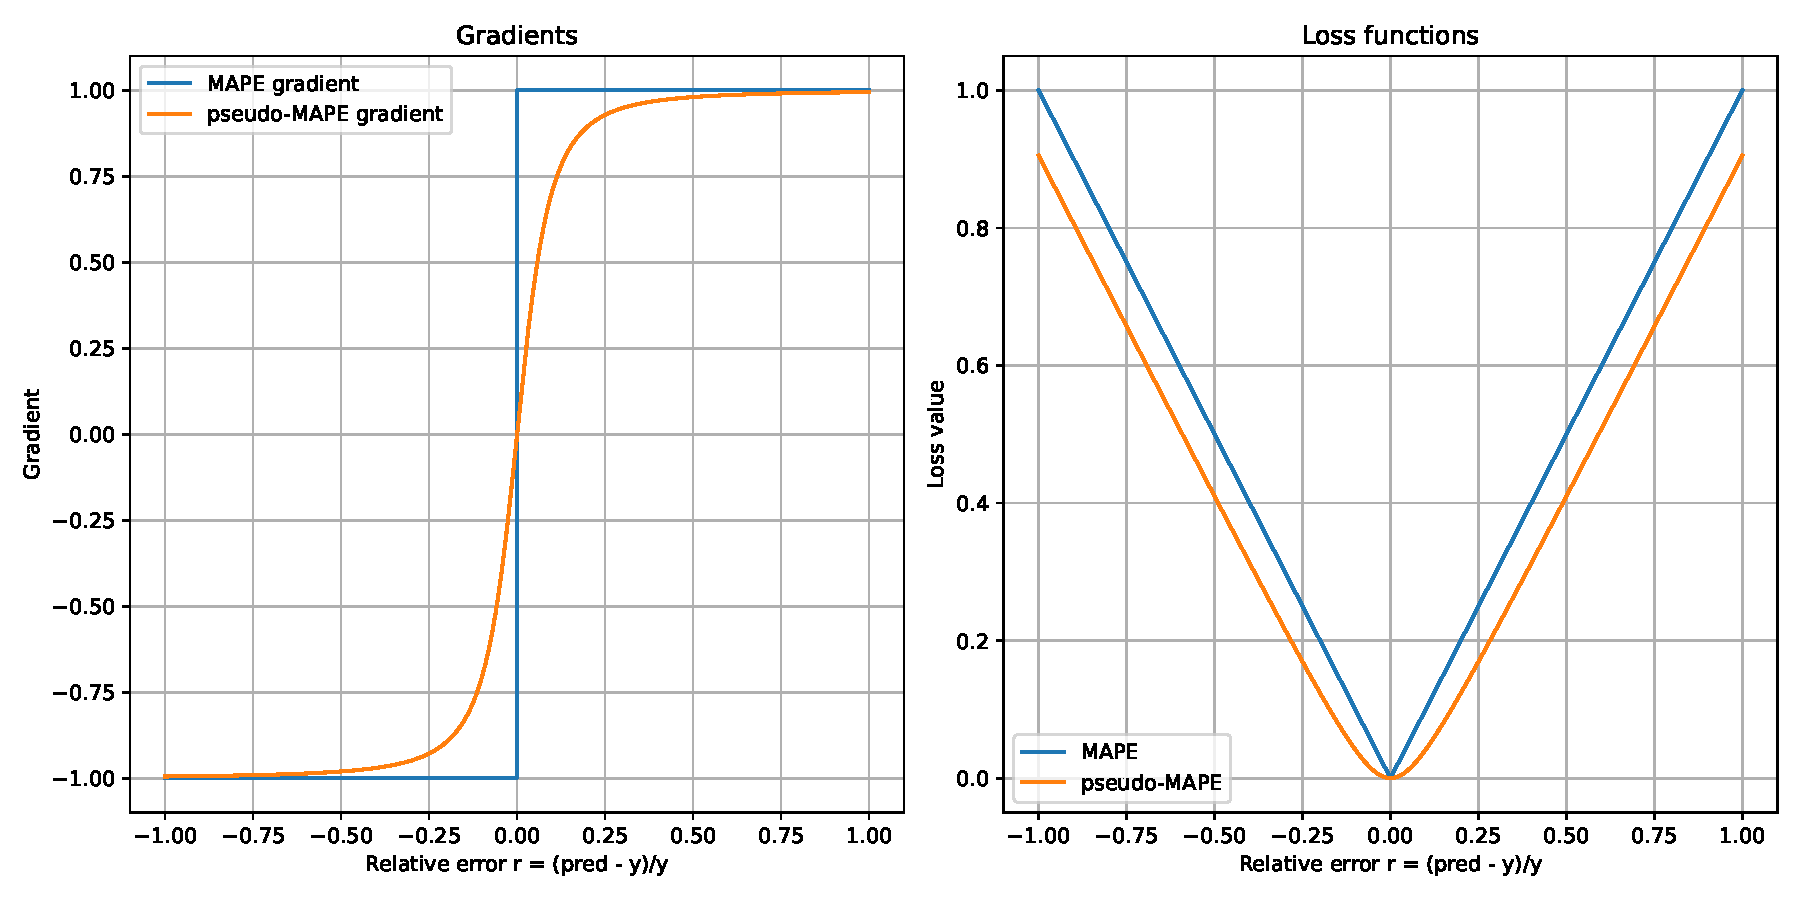
\includegraphics[width=1\textwidth]{bin/mape_vs_pseudo_mape.pdf}
\end{frame}

%--------------------------------------------------
\begin{frame}{Random Forest и Gradient Boosting}
    \begin{columns}[t,onlytextwidth]
        % ---------- Случайный лес ----------
        \column{0.48\textwidth}
        \begin{block}{Random Forest}
            \[
                f_{\mathrm{RF}}(x)=\frac{1}{B}\sum_{b=1}^{B} f^{(b)}(x)
            \]

            \begin{itemize}
                \item Разделение времён года
            \end{itemize}
        \end{block}

        % ---------- Градиентный бустинг ----------
        \column{0.48\textwidth}
        \begin{block}{Gradient Boosting}
            \[
                f_{(B)}(x)=f^{(0)}(x)+\nu\sum_{b=1}^{B} f^{(b)}(x)
            \]

            \begin{itemize}
                \item Последовательная обработка осадков из прошлого.
            \end{itemize}
        \end{block}
    \end{columns}

\end{frame}

%----------------------------------------------------------------------------------------------------------
% ============================================================
% Boosting frames (example – extend as needed)
% ============================================================

% --- first four bar plots (bar0–bar3) ----------------------------------------
\begin{frame}{Результаты: Gradient Boosting}
    \quadgraphics{bin/shap_plots/boosting/shap\_top10\_bar0.pdf}%
    {bin/shap_plots/boosting/shap\_top10\_bar1.pdf}%
    {bin/shap_plots/boosting/shap\_top100.pdf}%
    {bin/shap_plots/boosting/shap\_top101.pdf}%
\end{frame}

% % --- next two bar plots + overall summaries ----------------------------------
% \begin{frame}{Результаты: Gradient Boosting}
%     \quadgraphics
%     {bin/shap_plots/boosting/shap\_top102.pdf}%
%     {bin/shap_plots/boosting/shap\_top103.pdf}
% \end{frame}

% ============================================================
% Random‑Forest frames (mirror of above)
% ============================================================
\begin{frame}{Результаты: Random Forest}
    \quadgraphics{bin/shap_plots/forest_50/shap\_top10\_bar0.pdf}%
    {bin/shap_plots/forest_50/shap\_top10\_bar1.pdf}%
    {bin/shap_plots/forest_50/shap\_top100.pdf}%
    {bin/shap_plots/forest_50/shap\_top101.pdf}%
\end{frame}

% \begin{frame}{Результаты: Random Forest}
%     \quadgraphics{bin/shap_plots/forest/shap\_top100.pdf}%
%     {bin/shap_plots/forest/shap\_top101.pdf}%
%     {bin/shap_plots/forest/shap\_top102.pdf}%
%     {bin/shap_plots/forest/shap\_top103.pdf}
% \end{frame}

\begin{frame}{Результаты}
    \centering
    \begin{tabular}{
            l
            c
            c
            c
            c
        }
        \toprule
        \textbf{Model}    & \textbf{NSE} & \textbf{MAPE} & \textbf{RMSE} & \textbf{MAE} \\
        \midrule
        Random Forest     & -398.5       & 1355.1        & 60.654        & 36.755       \\
        Gradient Boosting & 0.470        & 27.009        & 2.216         & 0.853        \\
        \bottomrule
    \end{tabular}
\end{frame}


\begin{frame}{Результаты}
    \centering
    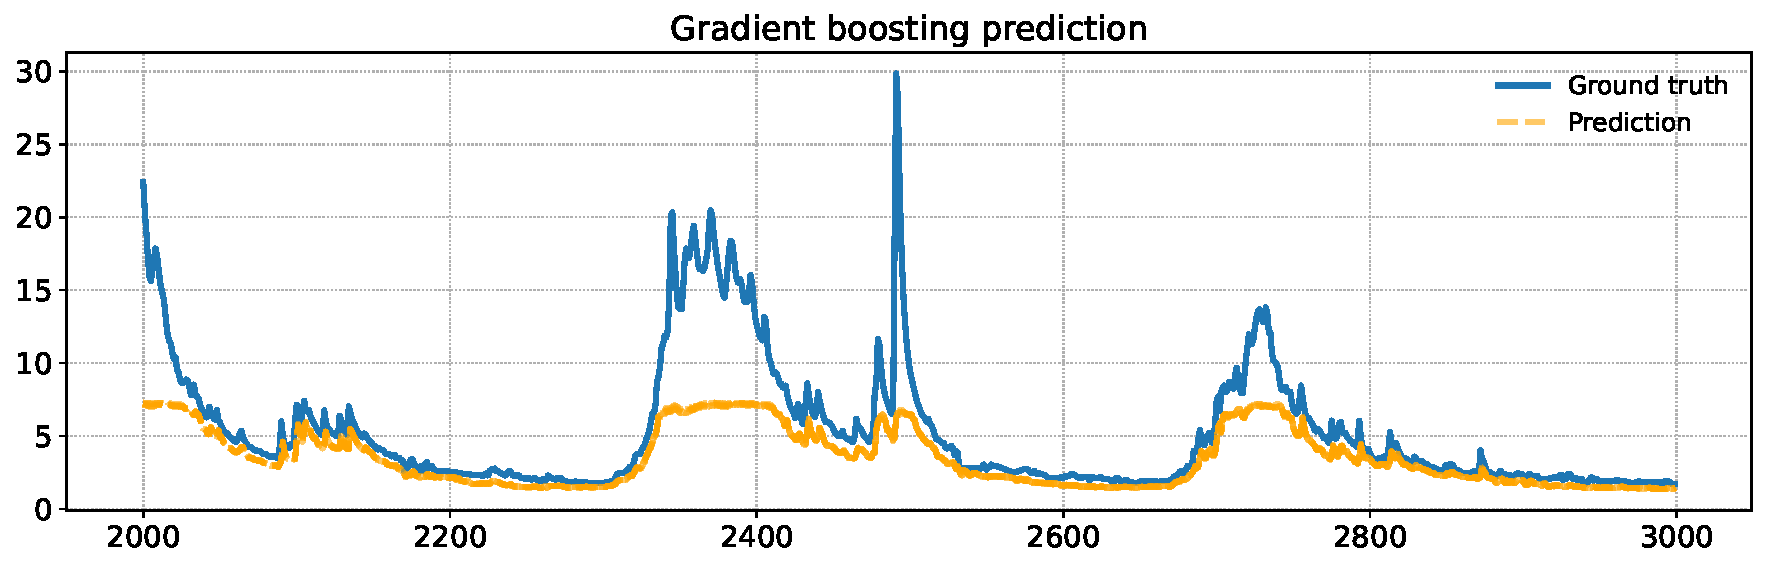
\includegraphics[width=\textwidth]{bin/Gradient_prediction.pdf}
    \vspace{0.3cm}      % adjust spacing as you like
    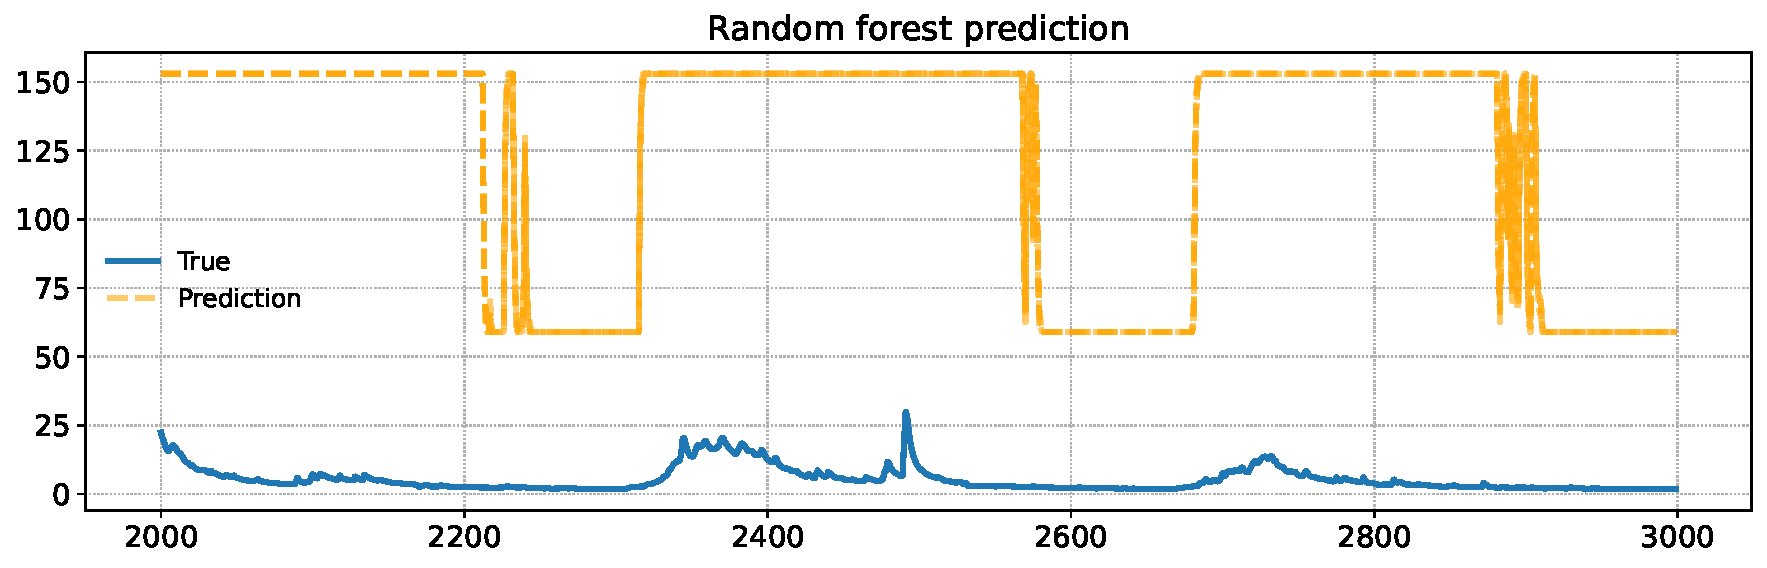
\includegraphics[width=\textwidth]{bin/forest_prediction.pdf}\par
\end{frame}

%------------------------------------------------------------------------------------
\begin{frame}{Заключение}
    \begin{itemize}
        \item Требуется анализ с использованием обширного датасета
        \item Модели внутри класса Gradient Boosting не проявляют эквифинальности
        \item Модели внутри класса Random Forest не проявляют эквифинальности
        \item Лучшие в классах Random Forest и Gradient Boosting модели выделяют разные признаки
    \end{itemize}
\end{frame}
%----------------------------------------------------------------------------------------------------------
\end{document}